\documentclass{article}
% PKGS START
\usepackage[utf8x]{inputenc}
\usepackage[english,russian]{babel}
\usepackage{cmap}
\usepackage{commath}
\usepackage{amsmath}
\usepackage{amsfonts}
\usepackage{mathtools}
\usepackage{amssymb} 
\usepackage{parskip}
\usepackage{titling}
\usepackage{color}
\usepackage{hyperref}
\usepackage{cancel}
\usepackage{enumerate}
\usepackage{graphicx}
\usepackage[a4paper, left=2.5cm, right=1.5cm, top=2.5cm, bottom=2.5cm]{geometry}
% PKGS END
% INIT START
\graphicspath{ {./images/} }
\setlength{\droptitle}{-3cm}
\hypersetup{
    colorlinks=true, %set true if you want colored links
    linktoc=all,     %set to all if you want both sections and subsections linked
    linkcolor=blue,  %choose some color if you want links to stand out
}

\pagenumbering{arabic}
% INIT END
\begin{document}
    \section{Отображение множеств.}

    \textbf{Определение 1.} Пусть имеются два множества $A$ и $B$. Говорят, что определено отображение множества $A$ в множество $B$, если каждому элементу $x$ из множества $A$ по некоторому правилу сопоставляется единственный элемент y множества $B$.\\
    $\forall x \in A\ \exists!\ y \in B$ по правилу $f$.
    
    \begin{figure}[h!]
    \centering
    
\includegraphics[scale=0.75]{2_1}
    \end{figure}

    Для обозначения отображения $f$ из $A$ в $B$ используют запись $f: A \rightarrow B$ или $A \xrightarrow[]{f} B$. Говорят, что отображение действует из $A$ в $B$. То, что элемент y является результатом действия $f$ на элемент $x$ обозначают $f: x \rightarrow y$ или $y = f(x)$.

    \textbf{Пример.}

    Пусть $A = \{$множество всех детей$\}$,\\
    $B = \{$множество всех мам$\}$,\\
    $C = \{$множество всех бабушек$\}$.

    Существует отображение $A$ в $B$, но не существует отображения $A$ в $C$.  
    
    \textbf{Пример.}
    
    Пусть правило $f$ действует следующим образом $f: x \rightarrow x^2$.
    
    Если $A = (0, 1)$, $B = [0, 1]$, то $f$ —-- отображение.
    
    Если $A = [0, 1]$, $B = (0, 1)$, то $f: A \rightarrow B$ —-- не отображение. 

    \textbf{Определение 2.} Множество $A$ чаще всего называется областью определения отображения $f (A = D_f)$, множество $B$ иногда называют областью значений.

    Имеются конкурирующие названия для $A$ и $B$: начало и конец отображения $f$ или источник и цель отображения $f$. 
    
    \textbf{Правила}, определяющие отображение, могут задаваться различными способами:

    \begin{enumerate}
        \item Формула. Пусть $A = B = \mathbb{R}$, $f: x \rightarrow x + 1$. Заметим, что если $A = B = \mathbb{N}$, то получим другое отображение.
        \item Словесное задание. $\phi: N \rightarrow \{0,1,2,...,9\}$, где $\phi(n)$ —-- $n$-ая цифра десятичной записи числа $\pi$. Об этом отображении мало что известно. Не ясно, например, одинаково ли часто встречаются различные цифры в записи числа $\pi$, нет ли достаточно длинных кусков записи, состоящих из одной цифры и т.п.
    \end{enumerate}

    \textbf{Определение 3.} Если $f: x \rightarrow y$, то элемент $y$ называется образом элемента $x$ при отображении $f$ или значением отображения $f$ в точке $x$.

    \textbf{Определение 4.} Множество тех элементов $y$ из $B$, для которых найдется такой элемент $x \in A$, что $f(x) = y$, называется образом множества $A$ при отображении $f$ и обозначается $f(A)$ или $Im f$.

    \[f(A) \overset{\mathrm{def}}{=} \{y \in B\ |\ y = f(x),\ x \in A\}\]

    \textbf{Пример.} $f: x \rightarrow x^2$. Если $A = [0, 1)$, $B = [0, 1]$, то $f(A) = [0, 1)$. $f(A) \neq B$.

    \textbf{Замечание.} Если $A_1 \subseteq A$, то образом подмножества $A_1$ назовем

    \[f(A_1) \overset{\mathrm{def}}{=} \{y \in B\ |\ y = f(x),\ x \in A_1\}\]

    \textbf{Лемма.} Докажем, что если $A_1 \subseteq A_2 \subseteq A$, то $f(A_1) \subseteq f(A_2)$.

    $\uparrow$ Рассмотрим произвольный $x \in A_1$, так как $A_1 \subseteq A_2$, то $x \in A_2$. Под действием отображения $f: x \in A_1 \rightarrow y = f(x) \in f(A_1)$. Но так как этот же $x \in A_2$, то этот же $y = f(x) \in f(A_2)$. Т.е. показали, что если произвольный $y \in f(A_1)$, то $y \in f(A_2)\ (f(A_1) \subseteq f(A_2))$. (важно, что для произвольного) $\downarrow$

    Мы выяснили, что $f(A)$ является подмножеством множества $B$, и вообще говоря, не совпадает с $B$.

    \textbf{Определение 5.} Если $f(A) = B$, то отображение $f$ называется наложением (отображением ``на`` или сюръекцией.

    \textbf{Пример.} $f: x \rightarrow x^2$. Если $A = (-1, 1)$, $B = [0, 1)$, то $f$ --— наложение, если $A = (-1, 1)$, $B = [0, 1]$, то $f$ не является наложением.

    \textbf{Определение 6.} Если $f: x \rightarrow y$, то элемент $x$ называется прообразом элемента $y$ при отображении $f$.

    Не у всякого $y \in B$ должен быть прообраз, например, если $y \in B \backslash f(A)$, то у него нет прообраза.

    \textbf{Важное замечание!} Отметим, что если отображение $f$ --— наложение, то у каждого $y$ есть прообраз (хотя бы один).

    Отображение $f$ дает для каждого $x$ единственный элемент $y = f(x)$, но вовсе не обязательно, чтобы только один $x$ при отображении $f$ перешёл в данный $y = f(x)$. Соберем вместе те элементы $x$ множества $A$, которые при отображении $f$ переходят в один и тот же элемент $y$ из $B$.

    \textbf{Определение 7.} Множество $f^{-1}(y) \overset{\mathrm{def}}{=} \{x \in A\ |\ f(x) = y\}$ --− называется полным прообразом элемента $y$.

    Отметим, что прообраз $y$ --— элемент, а полный прообраз —-- множество, хотя возможно, состоящее только из одного элемента.

    \begin{figure}[h!]
    \centering
    
\includegraphics[scale=0.75]{2_2}
    \caption{\label{fig:fig2}Здесь $f^{-1}(y) = \emptyset$}
    \end{figure}

    \textbf{Пример.}
    
    \begin{enumerate}
        \item $f: x \rightarrow x^2$. Если $A = \mathbb{R}$, $B = \mathbb{R}$. В этом примере число $4$ имеет два прообраза ($-2$ и $2$).
        \item Другой пример дает нам ортогональная проекция $\pi_l$ плоскости $\textrm{П}$ на прямую $l$, ставящая в соответствие каждой точке $x$ плоскости основание перпендикуляра, опущенного из $x$ на прямую $l$. Прообразы точки $y \in l$ заполняют целый перпендикуляр $p$ к прямой $l$, проходящий через точку $y:\ \pi_l^{-1}(y) = p$.
    \end{enumerate}

    \textbf{Определение 8.} Отображение $f: A \rightarrow B$ называется вложением (отображением ``в`` или инъекцией), если полный прообраз всякого элемента $y \in B$, т.е $f^{-1}(y)$ состоит не более чем из одного элемента. Т.е. если прообраз есть, то он один. Легко понять, что отображение $f$ является вложением $\Leftrightarrow \forall\ x_1$ и $x_2$ из $A:\ (x_1 \neq x_2) \Rightarrow (f(x_1) \neq f(x_2))$, т.е. вложение переводит различные элементы в различные.

    \textbf{Определение 9.} Если отображение $f: A \rightarrow B$ является одновременно вложением и наложением, то это отображение называется взаимно однозначным соответствием (биективным отображением или просто биекцией).

    \textbf{Пример (сводный пример).} При одном и том же правиле, задающем отображения, свойства отображения зависят от множеств $A$ и $B$.

    \begin{enumerate}
        \item Пусть $f:\ x \rightarrow x + 1$. Если $A = B = \mathbb{R}$, то отображение —-- биекция. Если $A = B = \mathbb{N}$, то отображение —-- вложение, но не наложение (у $y = 1$ нет прообраза).
        \item Пусть $f:\ x \rightarrow x^2$.\\
        Если $A = [0, 1]$, $B = (0, 1)$, то $f:\ A \rightarrow B$ --- не отображение;\\
        Если $A = (0, 1)$, $B = [0, 1)$, то отображение --- вложение, но не наложение (у $0$ нет прообраза);\\
        Если $A = (-1, 1)$, $B = [0, 1)$, то отображение --- наложение, но не вложение (у $\frac{1}{4}$ два прообраза $\frac{1}{2}$ и $-\frac{1}{2}$);\\
        Если $A = (0, 1)$, $B = (0, 1)$, то отображение --- биекция;
        \item Конечно, $f$ тоже важно! Пусть $A = [0, 1]$, $B = [0, 1]$. Если $f:\ x \rightarrow x^2$, то отображение —-- биекция, а если $f = 4(x - \frac{1}{2})^2$, то отображение наложение, но не вложение.
    \end{enumerate}

    \textbf{Замечание.} Легко понять, что если $f:\ A \rightarrow B$ --- вложение, то изменив конец отображения, $f:\ A \rightarrow f(A)$ превратим вложение $f$ в биекцию.

    Пусть теперь даны два отображения
    \[f:\ A \rightarrow B,\qquad g:\ B \rightarrow C\]

    \textbf{Определение 10.} Отображение из $A$ в $C$, определяемое правилом $x \rightarrow g(f(x))$ и получающееся последовательным выполнением отображений $f$ и $g$ называется композицией отображений $f$ и $g$ и обозначается $g \circ f$ (читается справа налево!). Итак
    \[g \circ f(x) = g(f(x))\]

    \subsection{Свойства композиции отображений.}
    
    \textbf{Свойство 1.} Композиция отображений $f$ и $g$, вообще говоря, зависит от порядка, в котором берутся отображения: $f \circ g \neq g \circ f$ даже тогда, когда отображение $f \circ g$ определено (отсутствие коммутативности для композиции отображений).

    1.1. Пусть отображения $f$ и $g$ заданы следующим образом (см. рисунок)

    \begin{figure}[h!]
    \centering
    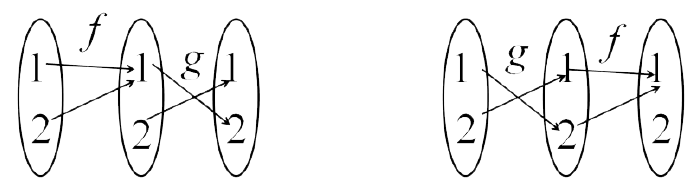
\includegraphics[scale=0.5]{2_3}
    \end{figure}

    Тогда $g \circ f(1) = 2,\ g \circ f(2) = 2$, а $f \circ g(1) = 1,\ f \circ g(2) = 1$.

    1.2. Отображение $x \rightarrow 2x^2$ дает пример композиции отображений $f:\ x \rightarrow x^2$ и $g:\ x \rightarrow 2x$. $g \circ f(x) = 2x^2$, но $f \circ g(x) = 4x^2$.

    \textbf{Свойство 2.} Пусть кроме отображений $f:\ A \rightarrow B$, $g:\ B \rightarrow C$ дано ещё одно отображение $h: C \rightarrow D$. Сквозное отображение из $A$ в $D$ получается двумя способами: на первом этапе мы образуем $g \circ f$, а потом действуем отображением $h$, или применяем вначале $f$, а потом $h \circ g$. На самом деле оба этих отображения совпадают:
    \[h \circ (g \circ f) = (h \circ g) \circ f\]
    (ассоциативность композиции отображений).

    $\uparrow h \circ (g \circ f)(x) = h(g \circ f(x)) = h(g(f(x))),\ (h \circ g) \circ f = h \circ g(f(x)) = h(g(f(x)))$, т.е. оба этих отображения определяются правилом: применим $f$, потом $g$, потом $h$. $\downarrow$

    Это свойство позволяет нам опустить скобки и писать просто $h \circ g \circ f$.

    % \begin{figure}[h!]
    % \centering
    % 
\includegraphics{2}
    % \caption{\label{fig:fig2}Разность и симметрическая разность множеств.}
    % \end{figure}

\end{document}